% Last Update: $Id$
\subsection{OPT\_IGMPPROXY - Proxy für Internet Group Management Protocol}
\configlabel{OPT\_IGMPPROXY}{OPTIGMPPROXY}

Die Deutsche Telekom AG bietet mittlerweile seit einigen Jahren VDSL25/50
(Bandbreite: 25/50 MBit/s) zusammen mit Entertain-Paketen an. Damit besteht die
Möglichkeit, Fernsehen über Internet (IPTV) zu empfangen.

Die Verteilung von IPTV erfolgt als Multicast, d.h. von einem Punkt zu einer
(geschlossenen) Gruppe. Zur Organisation vom Multicast-Gruppen ist das
Netzwerkprotokoll IGMP (Internet Group Management Protocol) notwendig. IGMP
(\altlink{http://de.wikipedia.org/wiki/IGMP}) bietet die Möglichkeit, dynamisch
Multicast-Gruppen zu verwalten. Die Verwaltung findet nicht in der Sende-Station
statt, sondern in den Routern, an denen Empfänger einer Multicast-Gruppe direkt
angeschlossen sind. IGMP bietet Funktionen, mit denen eine Station einem Router
mitteilt, dass sie Multicast-IP-Pakete einer bestimmten Multicast-Gruppe
empfangen will.

Die mitgelieferten Speedport-Router (derzeit W700V/W701V/W722) unterstützen
IGMP. Wer fli4l für IPTV statt Speedport-Router nutzen will, benötigt einen
IGMP-Proxy (\altlink{http://sourceforge.net/projects/igmpproxy/}) auf dem
fli4l-Router. OPT\_IGMPPROXY ist ein IGMP-Proxy für fli4l.

Diese Dokumentation zum OPT\_IGMP Paket beschreibt die Konfiguration von fli4l,
um VDSL und IPTV mit der mitgelieferten Set-Top-Box (STB) X300T/X301T bzw.
MR-303 hinter einem fli4l-Router zu betreiben. In dieser Beschreibung erfolgt
die Installation von IPTV über eine zusätzliche Netzwerkkarte.

\subsubsection{Voraussetzung}

Die Deutsche Telekom hat VDSL als VLAN eingeführt. In der Einführungsphase
(Startnetz) wurde nur ein VLAN-Tag (ID7) verwendet, über den der gesamte Traffic
floss. Nach der Umstellung (Zielnetz) auf zwei VLAN-Tags (ID7, ID8) bleibt der
Internet Traffic auf ID7 und der neue ID8 wird ausschließlich für den IPTV
Multicast-Traffic verwendet. Die Umstellung des VDSL Betriebs auf das Zielnetz
(zwei VLAN Tags ID7/ID8) ist nach derzeitigem Stand größtenteils abgeschlossen.


Hardware (neben Set-Top-Box und VDSL-Modem):
\begin{itemize}
   \item{HW für fli4l: Für VDSL 25/50 sollte es besser kein 486er mehr sein.
Falls es zu Bild-/Tonstörungen kommt kann das daran liegen, dass die eingesetzte
HW zu wenig Leistung hat.}
   \item{High-End-NICs (Beispiele: 3Com, Intel Pro100). Realtek-Chipsätze
stellen    eher das Low-End-Spektrum dar.}
\end{itemize}

Software:
\begin{itemize}
   \item{Paket: advanced\_networking}
   \item{Paket: dhcp\_client (für Zielnetz und Verwendung von ID8)}
\end{itemize}

Die Anpassung der Konfigurationsdateien (base.txt, dsl.txt,
advanced\_networking.txt, dhcp\_client.txt, dns\_dhcp.txt) wird im Folgenden
beschrieben.

\subsubsection{Hardware Setup}

Die Empfehlung für den Speedport-Router, die IPTV STB ohne weitere
Netzwerk-Elemente direkt an den Router anzuschließen, gilt natürlich auch für
den fli4l-Router. Falls dennoch Netzwerk-Knoten (Hub, Switch, Bridge, Gateway,
Router) zwischen IPTV Box und Router geschaltet werden, sollten diese
multicastfähig sein, um Störungen zu vermeiden.

Im Heimnetz werden i.d.R. keine Switche verwendet, die virtuelle Netze (VLAN)
voneinander trennen, um den restlichen Verkehr (ID7) vom IPTV Multicast-Traffic
(ID8) zu entlasten.

Deshalb wird hier als HW-Konfiguration eine separate NIC (Network Interface Card
= LAN- bzw. Ethernet-Karte) im fli4l verwendet, um die Set-Top-Box (STB) direkt
mit dem fli4l zu verbinden und das restliche Heimnetz vom Multicast-Traffic zu
entlasten und alle o.g. Probleme auszuschließen. Wer die 'Single'-NIC-Methode
bevorzugt sollte selbst wissen was er tut (das wird hier nicht weiter
beschrieben).

Anbei ein Diagramm, wie im genannten Beispiel der fli4l-Router
vom Standard-Router zum Router mit 3 NIC’s migriert wird:

\begin{itemize}
   \item{Standard-Konfiguration:
         \begin{itemize}
            \item{eth0 wird als NIC für das interne home/office LAN in base.txt
eingetragen}
            \item{In dsl.txt wird als DSL-Interface eth1 angegeben}
         \end{itemize}
         \begin{figure}[ht!]
         \centering
         \fontfamily{phv}\selectfont
VDSL-Modem~~~~~Fli4l-Router~~~~~~~~~~~~~~~~\\
         
\includegraphics[]{image001}\\
         ~~~~~~~~~~~~~~~~~~~~~~~~~~~~~~~~~~~~~~~~~~~~LAN-Schnittstelle
         \caption{Fli4l in der Standardkonfiguration}
         \label{fig:standardconfig}
         \end{figure}
      }
   \item{Erweiterte Konfiguration mit zusätzlicher IPTV NIC:
         \begin{itemize}
            \item{Nach Einbau der zusätzlichen NIC in den fli4l-Router wird
diese in base.txt als eth2 eingetragen.} \end{itemize}
         \begin{figure}[ht!]
         \centering
         \fontfamily{phv}\selectfont
~~~~~~~VDSL-Modem~~~~~Fli4l-Router~~~~~Schnittstelle zur IPTV-STB\\
         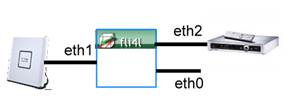
\includegraphics[]{image002}\\
         ~~~~~~~~~~~~~~~~~~~~~~~~~~~~~~~~~~~~~~~~~~~~LAN-Schnittstelle
         \caption{Fli4l in der IPTV-Konfiguration}
         \label{fig:iptvconfig}
         \end{figure}
      }
\end{itemize}


\subsubsection{VLAN-Konfiguration}

Eines vorweg: OPT\_IGMP ist nicht auf VLAN angewiesen. Vielmehr wird VLAN
derzeit von der Deutschen Telekom für VDSL verwendet und muss dafür vom Router
unterstützt werden. Ob VLAN für den Internet-Betrieb auch bei anderen Providern
(Arcor, Alice, etc...) benötigt wird, ist uns nicht bekannt.

Um VDSL25/50 von T-Home für den Internet-Betrieb zum Laufen zu bringen, muss die
NIC zum VDSL-Modem zwingend als VLAN-Interface konfiguriert werden - siehe auch
(\altlink{http://www.fli4l.de/fileadmin/doc/deutsch/html/fli4l-3.4.0/node30.html
}).

\vspace{3mm}
\emph{Ein Hinweis für alle, die nur das 'normale DSL' der Telekom, also ADSL,
ADSL2, ADSL2+ haben: VLAN wird nur von VDSL benötigt, nicht aber vom 'normalen
DSL'. Die VLAN-Konfiguration wird deshalb mit dem 'normalen DSL' nicht
funktionieren.}
\vspace{3mm}

Bei dem Vorhandensein von zwei VLAN-Tags (Zielnetz, siehe oben) wird der
traffic wie folgt aufgeteilt:

\begin{itemize}
   \item{VLAN ID7: Internet-Traffic}
   \item{VLAN ID8: IPTV Multicast-Traffic}
\end{itemize}

Damit läuft Internet-Traffic unabhängig vom IPTV-Traffic. Wesentlicher
Unterschied ist, dass für VLAN ID7 eine PPPoE-Einwahl erforderlich ist.
VLAN ID8 wird über einen DHCP-Server ohne Einwahl zur Verfügung gestellt.
In dieser Zielarchitektur gibt es keine Zwangstrennung nach 24h mehr.\\

Für VLAN ist folgende Konfiguration erforderlich (NICs wie im Abschnitt
Hardware-Setup angegeben):\\

\noindent \textbf{advanced\_networking.txt}

\begin{example}
\begin{verbatim}
VLAN_DEV_N='2'
VLAN_DEV_1_DEV='eth1’     # interface of VDSL-Modem; example: eth1
                          # In unserem Beispiel geht 'eth1' zum VDSL-Modem
VLAN_DEV_1_VID='7         # ID7 to support VLAN for internet
VLAN_DEV_2_DEV='eth1’     # interface of VDSL-Modem; example: eth1
                          # In unserem Beispiel geht 'eth1' zum VDSL-Modem
VLAN_DEV_2_VID='8’        # ID8 to support VLAN for IPTV
\end{verbatim}
\end{example}

\noindent Die Virtual-NIC eth1.7 muss in die DSL-Konfiguration eintragen
werden:\\

\noindent \textbf{dsl.txt}

\begin{example}
\begin{verbatim}
PPPOE_ETH='eth1.7'        # eth<nummer der karte zum vdsl-modem>.7'
                          # Bsp 'eth1.7'
\end{verbatim}
\end{example}

\noindent Für die Virtual-NIC eth1.8 benötigen wir einen dhcp\_client, da VLAN
ID8 über einen DHCP-Server ohne Einwahl zur Verfügung gestellt wird.\\

\noindent \textbf{dhcp\_client}

\begin{example}
\begin{verbatim}
OPT_DHCP_CLIENT='yes'
DHCP_CLIENT_TYPE='dhcpcd'
DHCP_CLIENT_INTERFACES='IP_NET_3_DEV' # listen on interface eth1.8
DHCP_CLIENT_USEPEERDNS='no'
DHCP_CLIENT_HOSTNAME=''
\end{verbatim}
\end{example}

Seit Fli4l V3.3 kann für das Interface nicht mehr \texttt{eth1.8} angegeben
werden, sondern es muss der Eintrag \texttt{IP\_NET\_x\_DEV} verwendet werden,
der für das Interface in base.txt definiert wurde; hier
\texttt{IP\_NET\_3\_DEV}.\\

\noindent Optional:\\
Falls die verwendete NIC mit der MTU-Größe Probleme hat, muss der MTU-Wert über
den Parameter DEV\_MTU angepasst werden. Im Test zeigten Intel Pro/100 (e100)
und auch eine 3-Com-Karte keine Probleme, andere User berichten, dass bei der
3Com '3c59x' der MTU-Wert auf 1496 angepasst werden muss.

\begin{example}
\begin{verbatim}
DEV_MTU_1=''              # Adjust MTU size of NIC on VDSL-Modem
                          # Example: DEV_MTU_1='eth1 1496'
\end{verbatim}
\end{example}

Jetzt sind noch die Konfigurationsdateien base.txt und dns\_dhcp.txt anzupassen,
wie im nächsten Kapitel beschrieben.\\

\subsubsection{Konfiguration einer zusätzlichen NIC für IPTV}

In base.txt und dns\_dhcp.txt muss die Konfiguration für VLAN und für die zweite
NIC angepasst werden.\\

\noindent Zweite NIC für IPTV eintragen:\\

\begin{example}
\begin{verbatim}
NET_DRV_N='2'
NET_DRV_1='via-rhine'     # 1. NIC für als LAN-Schnittstelle
NET_DRV_2='3c59x'         # 2. NIC – hier 3Com für IPTV SetTopBox
\end{verbatim}
\end{example}

Jetzt muss der Adressraum für die zweite NIC festgelegt werden. Hier wird fürs
LAN 192.168.2.0/24 und für die zweite NIC 192.168.3.0/24 verwendet. Außerdem
werden Einträge für die Virtual-NICs eth1.7 und eth1.8 benötigt:\\

\begin{example}
\begin{verbatim}
IP_NET_N='4'
IP_NET_1='192.168.2.1/24'           # home/office LAN
IP_NET_1_DEV='eth0'
IP_NET_2='192.168.3.1/24'           # iptv LAN
IP_NET_2_DEV='eth2'
IP_NET_3='dhcp'                     # dhcp client - IP ueber dhclient
IP_NET_3_DEV='eth1.8'
IP_NET_3_MAC='00:40:63:da:cf:32'    # neue MAC/nicht MAC von eth1
IP_NET_4='dhcp'                     # eth1.7 zum modem
IP_NET_4_DEV='eth1.7'
IP_NET_4_MAC='00:40:63:da:cf:33'    # neue MAC/nicht MAC von eth1
\end{verbatim}
\end{example}

Wichtig ist auch die Änderung die MAC-Adressen für eth1.7 und eth1.8, welche
nicht mit eth1 übereinstimmen dürfen, da sonst – abhängig vom VDSL-Net der DTAG
– ggf. Störungen nach der Zwangstrennung auftreten können.

Für die neue NIC muss der Zugriff auf das Internet natürlich genauso
funktionieren, wie für die erste NIC. Dazu sind weitere Einstellungen
notwendig:\\

\begin{example}
\begin{verbatim}
PF_INPUT_1='IP_NET_1 ACCEPT'
PF_INPUT_2='IP_NET_2 ACCEPT'
PF_INPUT_3='any 224.0.0.0/4 ACCEPT'
[...]
PF_FORWARD_3='any 224.0.0.0/4 ACCEPT'
PF_FORWARD_5='IP_NET_1 ACCEPT'
PF_FORWARD_6='IP_NET_2 ACCEPT'
[...]
PF_POSTROUTING_1='IP_NET_1 MASQUERADE'
PF_POSTROUTING_2='IP_NET_2 MASQUERADE'
\end{verbatim}
\end{example}

Damit später auch eine dynamische DHCP-Adressierung an der neuen IPTV-NIC
klappt und die SetTop-Box mit einem Namen angesprochen werden kann, sind noch
folgende Einstellungen in dns\_dhcp.txt erforderlich:\\

\begin{example}
\begin{verbatim}
HOST_10_NAME='igmp'
HOST_10_IP4='192.168.3.1'
HOST_11_NAME='iptv'
HOST_11_IP4='192.168.3.4'
HOST_11_MAC='00:D0:E0:93:49:34'         # MAC Adr T-Home X300T
[...]
DHCP_RANGE_2_NET='IP_NET_2'
DNSDHCP_RANGE_2_START='192.168.3.10'
DNSDHCP_RANGE_2_END='192.168.3.20'
DNSDHCP_RANGE_2_DNS_SERVER1=''
DNSDHCP_RANGE_2_DNS_SERVER2=''
DNSDHCP_RANGE_2_NTP_SERVER=''
DNSDHCP_RANGE_2_GATEWAY=''
\end{verbatim}
\end{example}

Am Besten ist es, nach der Konfiguration der neuen NIC, diese erst einmal an einen
PC zu hängen um zu sehen ob man über die neue NIC auch ins Internet kommt. Ist
der Test erfolgreich, sollte die neue zweite NIC richtig konfiguriert sein.

\subsubsection{IGMP-Funktion}

Beim Booten des fli4l-Routers werden die Parameter der config-Datei proxy.txt in
die Konfigurationsdatei /etc/igmpproxy.conf geschrieben, welche beim Start des
Programms igmpproxy eingelesen werden.

Entgegen den früheren opt\_igmp Versionen, wird der IGMP-Proxy jetzt einmalig
beim Booten des Routers gestartet und läuft dann solange eine physikale
Verbindung zum Internet besteht. Der IGMP-Proxy wird weder durch die 24h
Zwangstrennung, noch durch ein manuelles trennen und verbinden des
Internet-Traffics beeinflusst.

\subsubsection{IGMP-Konfiguration}

\begin{description}

\config{OPT\_IGMPPROXY}{OPT\_IGMPPROXY}{}

Mit \var{'yes'} wird das IGMP Proxy Paket aktiviert. Die Einstellung \var{'no'}
deaktiviert das Paket komplett.

\config{IGMPPROXY\_DEBUG}{IGMPPROXY\_DEBUG}{IGMPPROXYDEBUG}

Mit \var{'yes'} können Meldungen des IGMP Proxies ins syslog ausgegeben werden.

\config{IGMPPROXY\_DEBUG2}{IGMPPROXY\_DEBUG2}{IGMPPROXYDEBUG2}

Mit \var{'yes'} kann das Loglevel des IGMP Proxies erhöht werden.

\config{IGMPPROXY\_QUICKLEAVE\_ON}{IGMPPROXY\_QUICKLEAVE\_ON}{
IGMPPROXYQUICKLEAVEON}

Mit Quickleave kann die Last im Upstream-Link gesenkt werden. Falls der
Parameter mittels \var{'yes'} eingeschaltet wird, führt dies dazu, dass der
Multicast nach einem Kanalwechsel schneller abbestellt und so die Last im
Downstream gesenkt wird, indem sich der IGMP-Proxy wie ein Receiver verhält.

Gibt es 2 STBen und sehen diese dasselbe Programm, dann kann es (mit Quickleave
= yes) passieren, dass beim Umschalten des Programms von einer STB bei der
zweiten STB das Programm unterbrochen wird. Beim Einsatz von nur einer STB kann
Quickleave gefahrlos eingeschaltet werden (yes).

\begin{example}
\begin{verbatim}
IGMPPROXY_QUICKLEAVE_ON='yes'      # Quickleave-Modus einschalten
                                   # yes or no; Default: yes
\end{verbatim}
\end{example}

\config{IGMPPROXY\_UPLOAD\_DEV}{IGMPPROXY\_UPLOAD\_DEV}{IGMPPROXYUPLOADDEV}

Für den IPTV-Betrieb benötigt der IGMP-Proxy ein Upstream- und ein
Downstream-Interface. Das Upstream-Interface ist die Schnittstelle mit der NIC,
an der das VDSL-Modem hängt. Diese sollte i.d.R. immer gleich bleiben.

Mit der Trennung von IPTV auf ID8 muss natürlich auch in der Konfiguration für
den IGMP-Proxy eth1.8 statt bisher ppp0 eingetragen werden, womit die Umstellung
Startznetz (nur ID7) auf das Zielnetz (mit ID7/8) komplett ist.

\begin{example}
\begin{verbatim}
IGMPPROXY_UPLOAD_DEV='eth1.8'      # Upstream Interface; Default: ppp0
                                   # eth1.8 für T-Home/VDSL mit id7/id8
\end{verbatim}
\end{example}

\config{IGMPPROXY\_DOWNLOAD\_DEV}{IGMPPROXY\_DOWNLOAD\_DEV}{IGMPPROXYDOWNLOADDEV
}

Die Schnittstelle des Downstream-Interfaces (NIC zur IPTV SetTop-Box) ist hier
abhängig von der HW-Konfiguration einzutragen. Für fli4l mit zweiter NIC – wie
in diesem Dokument beschrieben - ist eth2 das Interface zur SetTop-Box.

\begin{example}
\begin{verbatim}
IGMPPROXY_DOWNLOAD_DEV='eth2'      # Downstream Interface
\end{verbatim}
\end{example}

\config{IGMPPROXY\_ALT\_N}{IGMPPROXY\_ALT\_N}{IGMPPROXYALTN}

Mit diesem Parameter wird die Anzahl der Adressbereiche für Multicast Streams
festgelegt.

\config{IGMPPROXY\_ALT\_x\_NET}{IGMPPROXY\_ALT\_x\_NET}{IGMPPROXYALTxNET}

Mit dem Parameter IGMPPROXY\_ALT\_x\_NET werden Adressbereiche für
Multicast-Traffic festgelegt, welche Ihren Ursprung außerhalb des Heim-Netzwerks
haben, sowie der lokale Adressbereich, an dem die STB hängt.

\begin{example}
\begin{verbatim}
IGMPPROXY_ALT_N='3'                        # Anzahl der Multicast Sourcen
IGMPPROXY_ALT_1_NET='239.35.0.0/16'        # IPTV streams - immer benoetigt
IGMPPROXY_ALT_2_NET='217.0.119.0/24'       # Erforderlich fuer T-Home
IGMPPROXY_ALT_3_NET='193.158.34.0/23'      # Erforderlich fuer T-Home
                                           # vor Mai 2013 '193.158.35.0/24'
# IGMPPROXY_ALT_4_NET='192.168.3.0/24'     # Adressraum IPTV SetTop-Box/nicht
                                           # mehr notwendig
\end{verbatim}
\end{example}

\config{IGMPPROXY\_WLIST\_N}{IGMPPROXY\_WLIST\_N}{IGMPPROXYWLISTN}

Mit diesem Parameter wir die Anzahl der Whitelists für die IGMP Reports
festgelegt.

\config{IGMPPROXY\_WLIST\_x\_NET}{IGMPPROXY\_WLIST\_x\_NET}{IGMPPROXYWLISTxNET}:\newline

Bei IGMPv3 können alle Adressen in einem Report zusammengefasst werden
(\altlink{
http://grinch.itg-em.de/entertain/artikel/zielnetzarchitektur-und-igmpproxy/}).
Dieser wird dann komplett ignoriert, was dazu führt, dass der IGMP Querier
irgendwann sämtlichen Multicasttraffic abschaltet, da er denkt, dieser würde
nicht mehr benötigt. Um dies zu verhindern wurde die Konfiguration von
whitelists erlaubt. Nur Multicastgruppen in dieser Liste werden dann auch auf
WAN-Seite angefordert.

\begin{example}
\begin{verbatim}
IGMPPROXY_WLIST_N='1'                          # Anzahl der Multicast Sourcen
IGMPPROXY_WLIST_1_NET='239.35.0.0/16'         # IPTV streams - immer benoetigt
                                               # siehe oben
\end{verbatim}
\end{example}

\end{description}

\subsubsection{Änderungen in anderen Config-Dateien}

Seit Revision 32955 ist es nicht mehr notwendig, die Firewall für den IGMP Proxy
und die Multicast Streams anzupassen, wenn in der base.txt die  Standardregeln
für die Firewall aktiviert sind (\var{PF\_INPUT\_ACCEPT\_DEF='yes'} und
\var{PF\_FORWARD\_ACCEPT\_DEF='yes'}). Das Startskript fügt dann automatisch
die notwendigen Regeln ein, wenn \var{OPT\_IGMPPROXY='yes'} gesetzt ist.

Im Detail handelt es sich um zwei Regeln, die in der INPUT Kette eingetragen
werden, damit die eingehenden Nachrichten den IGMP Proxy erreichen:

\begin{example}
\begin{verbatim}
Chain INPUT (policy DROP 0 packets, 0 bytes)
 pkts bytes target   prot opt in   out   source         destination
 [...]
    0     0 ACCEPT   all  --  *    *     0.0.0.0/0      224.0.0.1     \
    /* automatically added for IGMP Proxy */

    0     0 ACCEPT   all  --  *    *     0.0.0.0/0      224.0.0.22    \
    /* automatically added for IGMP Proxy */
 [...]
\end{verbatim}
\end{example}

Und außerdem eine Regel in der FORWARD Kette, die erlaubt, dass die eingehenden
Multicast Streams auch zum Media Receiver weitergeleitet werden:

\begin{example}
\begin{verbatim}
Chain FORWARD (policy DROP 0 packets, 0 bytes)
 pkts bytes target   prot opt in   out   source         destination
 [...]
    0     0 ACCEPT   all  --  *    *     0.0.0.0/0      239.35.0.0/16  \
    /* automatically added for IPTV streams */
 [..]
\end{verbatim}
\end{example}

Sofern man die Standardregeln nicht aktiviert sind, müssen manuell mindestens
die folgenden Regeln eingefügt werden.

\begin{example}
\begin{verbatim}
PF_INPUT_x='any 224.0.0.1/32 ACCEPT'
PF_INPUT_x='any 224.0.0.22/32 ACCEPT'
[...]
PF_FORWARD_x='any 239.35.0.0/16 ACCEPT'
\end{verbatim}
\end{example}

\achtung{Hinweis: Gegenüber früheren Versionen der Dokumentation wurden die
   Regeln auf die tatsächlich notwendigen Netze eingeschränkt. Sofern das IPTV
   nicht laufen sollte, nehmen wir gerne Hinweise auf zusätzlich notwendige
   Netze entgegen.}

\achtung{WICHTIG!
Ab Ende Mai 2013 hat die Telekom für Entertain neue (classless) Routen
eingeführt
(\altlink{http://www.onlinekosten.de/forum/showthread.php?t=116415&page=38}).
Der Grund dafür scheint wohl zu sein, das jetzt mehr als 256 Sender bzw.
Adressen benutzt werden. Damit sendet der DHCP-Server dhcp-routen, die nicht
mehr im bisherigen Subnetz enthalten sind. Solange die Telekom nicht ihr
iptv-server-subnetz (193.158.34.0/23) wechselt, kann eine statische route fuer
das vlan8-interface anlegt werden, um diese Änderung zu berücksichtigen, da
sonst multicast nicht mehr funktioniert.}

Lösung: In base.txt muss ein zusätzliche Route angegeben werden.

\begin{example}
\begin{verbatim}
IP_ROUTE_N='1'
IP_ROUTE_1='193.158.34.0/23 eth1.8'
\end{verbatim}
\end{example}
